\chapter{Debug Module (DM)} \label{dm}

\begin{steps}{The Debug Module implements a translation interface between abstract debug
    operations and their specific implementation. It might support the following
    operations:}
\item Give the debugger necessary information about the implementation. (Required)
\item Allow any individual hart to be halted and resumed. (Required)
\item Provide status on which harts are halted. (Required)
\item Provide read and write access to a halted hart's GPRs. (Required)
\item Provide access to a reset signal that allows debugging from the very
    first instruction after reset. (Required)
\item Provide a mechanism to allow debugging harts immediately out of reset
      (regardless of the reset cause). (Optional)
\item Provide access to other hart registers. (Optional)
\item Provide a Program Buffer to force the hart to execute arbitrary instructions. (Optional)
\item Allow multiple harts to be halted, resumed, and/or reset at the same time. (Optional)
\item Allow memory access from a hart's point of view. (Optional)
\item Allow direct System Bus Access. (Optional)
\end{steps}

In order to implement memory access, a target must implement at least one of
Program Buffer, System Bus Access, or Abstract Access Memory command
mechanisms.

A single DM can debug up to $2^{20}$ harts.

\section{Debug Module Interface (DMI)} \label{dmi}

Debug Modules are slaves to a bus called the Debug Module Interface (DMI). The
master of the bus is the Debug Transport Module(s).
The Debug Module Interface can be a trivial bus with one master and one slave,
or use a more full-featured bus like TileLink or the AMBA Advanced Peripheral
Bus. The details are left to the system designer.

The DMI uses between 7 and 32 address bits.  It supports read and write
operations.  The bottom of the address space is
used for the first (and usually only) DM. Extra space can be used for custom
debug devices, other cores, additional DMs, etc. If there are additional DMs
on this DMI, the base address of the next DM in the DMI address space is given
in \Rnextdm.


The Debug Module is controlled via register accesses to its DMI address space.

\section{Reset Control} \label{reset}

The Debug Module controls a global reset signal, \Fndmreset
(non-debug module reset),
which can reset, or hold in reset, every component in the platform,
except for the Debug Module and Debug Transport Modules.
Exactly what is affected by this reset is implementation dependent, as long as
it is possible to debug programs from the first instruction executed.
The Debug Module's own state and registers should only be
reset at power-up and while
\Fdmactive in \Rdmcontrol is 0.
The halt state of harts should be
maintained across system reset provided that \Fdmactive is 1,
although trigger CSRs may be cleared.

Due to clock and power domain crossing issues,
it may not be possible to perform arbitrary DMI accesses across
system reset.
While \Fndmreset or any external reset is asserted, the only supported DM
operation is accessing \Rdmcontrol. The behavior of other accesses is
undefined.

There is no requirement on the duration of the assertion of \Fndmreset.
The implementation must ensure that a write of \Fndmreset to 1 followed by
a write of \Fndmreset to 0 triggers system reset. The system may take
an arbitrarily long time to come out of reset, as reported by \Fallunavail,
\Fanyunavail, or other implementation specific indicators.

When harts have been reset, they must set a sticky {\tt havereset} state bit.
The conceptual {\tt havereset} state bits can be read for selected harts in
\Fanyhavereset and \Fallhavereset in \Rdmstatus.
These bits must be set regardless of the cause of the reset.
The {\tt havereset} bits for the selected harts
can be cleared by writing 1 to \Fackhavereset in \Rdmcontrol.
The {\tt havereset} bits may or may not be cleared 
when \Fdmactive is low.

\section{Selecting Harts} \label{selectingharts}

Up to $2^{20}$ harts can be connected to a single DM. The debugger
selects a hart, and then subsequent halt, resume, reset, and debugging
commands are specific to that hart.

To enumerate all the harts, a debugger must first determine {\tt HARTSELLEN}
by writing  all ones to \Fhartsel (assuming the maximum size) and reading back
the value to see which bits were actually set.  Then it selects each hart
starting from 0 until either \Fanynonexistent in \Rdmstatus is 1, or the
highest index (depending on {\tt HARTSELLEN}) is reached.

The debugger can discover the mapping between hart indices and
\Rmhartid by using the interface to read \Rmhartid, or by
reading the system's Device Tree.

\subsection {Selecting a Single Hart}

All debug modules must support selecting a single hart.
The debugger can select a hart by writing its index to \Fhartsel.
Hart indexes start at 0 and are contiguous until the final index.

\subsection {Selecting Multiple Harts} \label{hartarraymask}

Debug Modules may implement a Hart Array Mask register to allow selecting
multiple harts at once. The Nth bit in the Hart Array Mask register applies to
the hart with index N. If the bit is 1 then the hart is selected.  Usually a DM
will have a Hart Array Mask register exactly wide enough to select all the
harts it supports, but it's allowed to tie any of these bits to 0.

The debugger can set bits in the hart array mask register using \Rhawindowsel
and \Rhawindow, then apply actions to all selected harts by setting \Fhasel. If
this feature is supported, multiple harts can be halted, resumed, and reset
simultaneously.

Only the actions initiated by \Rdmcontrol can apply to multiple harts
at once, Abstract Commands apply only to the hart selected by
\Fhartsel.

\section{Run Control} \label{runcontrol}

For every hart, the Debug Module contains 4 conceptual bits of state: halt
request, resume request, halt-on-reset request,  and hart reset.
(The hart reset and halt-on-reset request bits are optional.)
These bits all reset to 0. A debugger can write them for the currently selected
harts through \Fhaltreq, \Fresumereq, \Fsetresethaltreq/\Fclrresethaltreq and \Fhartreset in \Rdmcontrol.
In addition the DM receives halted, running, and resume ack signals from each
hart.

When a running hart receives a halt request, it responds by halting and
asserting its halted signal. The halted signals of all selected harts are
reflected in the \Fallhalted and \Fanyhalted bits. \Fhaltreq is ignored by
halted harts.

When a halted hart receives a resume request, it responds by resuming, clearing
its halted signal, and asserting its running signal and resume ack signals. The
resume ack signal is lowered when the resume request is deasserted.  These
status signals of all selected harts are reflected in \Fallresumeack,
\Fanyresumeack, \Fallrunning, and \Fanyrunning. \Fresumereq is ignored by
running harts.

When halt or resume is requested, a hart must respond in
less than one second, unless it is unavailable.
(How this is implemented is not further specified. A few
clock cycles will be a more typical latency).

The DM can implement optional halt-on-reset bits for each hart,
which it indicates by setting \Fhasresethaltreq to 1.
This means the DM implements the \Fsetresethaltreq and \Fclrresethaltreq bits.
Writing 1 to \Fsetresethaltreq sets the halt-on-reset request bit for each
selected hart.
When a hart's halt-on-reset request bit is set, the hart will immediately enter
debug mode on the next deassertion of its reset. This is true regardless of
whether or not the hart's reset is caused by the DM's
\Fndmreset/\Fhartreset signals.
The hart's halt-on-reset request bit remains set
until cleared by the debugger writing 1 to \Fclrresethaltreq
while the hart is selected, or by debug module reset.

\section{Abstract Commands} \label{abstractcommands}

The DM supports a set of abstract commands, most of which
are optional. Depending on the implementation, the debugger may
be able to perform
some abstract commands even when the selected hart is not halted.
Debuggers can only determine which abstract commands
are supported by a given hart in a given state by attempting them
and then looking at \Fcmderr in \Rabstractcs to see if they were successful.

Debuggers execute abstract commands by writing them to \Rcommand.
Debuggers can determine whether an abstract command is complete by
reading \Fbusy in \Rabstractcs.
If the command takes arguments, the debugger
must write them to the {\tt data} registers before writing to \Rcommand. If a
command returns results, the Debug Module must ensure they are placed
in the {\tt data} registers before \Fbusy is cleared.
Which {\tt data} registers are used for the arguments is
described in Table~\ref{tab:datareg}.  In all cases the least-significant word
is placed in the lowest-numbered {\tt data} register. The argument width
depends on the command being executed, and is MXLEN where not explicitly
specified.

\begin{table}[htp]
    \centering
    \caption{Use of Data Registers}
    \label{tab:datareg}
    \begin{tabulary}{\textwidth}{|r|l|l|l|}
        \hline
        Argument Width & arg0/return value & arg1 & arg2 \\
        \hline
        32 & \Rdatazero & {\tt data1} & {\tt data2} \\
        \hline
        64 & \Rdatazero, {\tt data1} & {\tt data2}, {\tt data3} & {\tt data4}, {\tt data5} \\
        \hline
        128 & \Rdatazero--{\tt data3} & {\tt data4}--{\tt data7} & {\tt data8}--{\tt data11} \\
        \hline
    \end{tabulary}
\end{table}

\subsection{Abstract Command Listing}

This section describes each of the different abstract commands
and how their fields should be interpreted when
they are written to \Rcommand.

Each abstract command is a 32-bit value. The top 8 bits contain \Fcmdtype which
determines the kind of command. Table~\ref{tab:cmdtype} lists all commands.

\begin{table}[htp]
    \centering
    \caption{Meaning of \Fcmdtype}
    \label{tab:cmdtype}
    \begin{tabulary}{\textwidth}{|r|l|l|l|}
        \hline
        \Fcmdtype & Command & Page \\
        \hline
        0 & Access Register Command & \pageref{access register} \\
        \hline
        1 & Quick Access & \pageref{quick access} \\
        \hline
        2 & Access Memory Command & \pageref{access memory} \\
        \hline
    \end{tabulary}
\end{table}

\input{abstract_commands.tex}

\begin{table}[htp]
    \centering
    \caption{Abstract Register Numbers}
    \label{tab:regno}
    \begin{tabulary}{\textwidth}{|r|l|}
        \hline
        0x0000 -- 0x0fff & CSRs. The ``PC'' can be accessed here through \Rdpc.
        \\
        \hline
        0x1000 -- 0x101f & GPRs \\
        \hline
        0x1020 -- 0x103f & Floating point registers \\
        \hline
        0xc000 -- 0xffff & Reserved for non-standard extensions and internal
        use. \\
        \hline
    \end{tabulary}
\end{table}

\section{Program Buffer} \label{programbuffer}

To support executing arbitrary instructions on a halted hart,
a Debug Module can include a Program Buffer that a debugger
can write small programs to. Systems
that support all necessary functionality using abstract commands
only may choose to omit the Program Buffer.

A debugger can write a small program to the Program Buffer, and then
execute it exactly once with the Access Register Abstract Command,
setting the \Fpostexec bit in \Rcommand.
The debugger can write whatever program it likes (including jumps out of the
Program Buffer), but the program must end with
{\tt ebreak} or {\tt c.ebreak}. To save hardware, an implementation may support
an implied {\tt ebreak} that is executed when a hart runs off the end of the
Program Buffer. This is indicated in \Fimpebreak. With this feature, a Program
Buffer of just 2 32-bit words can offer efficient debugging.

If \Fprogbufsize is 1, \Fimpebreak must be 1. It is possible that the Program
Buffer can hold only one 32- or 16-bit instruction, so the debugger must only
write a single instruction in this case, regardless of its size.
This instruction can be a 32-bit
instruction, or a compressed instruction in the lower 16 bits accompanied by a
compressed {\tt nop} in the upper 16 bits.

\begin{commentary}
    The slightly inconsistent behavior with a Program Buffer of size 1 is to
    accommodate hardware designs that prefer to stuff instructions directly
    into the pipeline when halted, instead of having the Program Buffer exist
    in the address space somewhere.
\end{commentary}

If the debugger executes a program that does not
terminate with an {\tt ebreak} instruction, the hart will remain in Debug Mode
until it is reset.

While these programs are executed, the hart does not leave Debug Mode (see
Section~\ref{debugmode}).  If an exception is encountered during execution of
the Program Buffer, no more instructions are executed, the hart remains in Debug
Mode, and \Fcmderr is set to 3 ({\tt exception error}).  If the debugger
executes a program that doesn't terminate, then it loses control of the hart.

Executing the Program Buffer may clobber \Rdpc. If that is the case, it must be
possible to read/write \Rdpc using an abstract command with \Fpostexec not set.
The debugger must attempt to save \Rdpc between halting and
executing a Program Buffer, and then restore \Rdpc before leaving Debug Mode.

\begin{commentary}
    Allowing Program Buffer execution to clobber \Rdpc allows for direct
    implementations that don't have a separate PC register, and do need to use
    the PC when executing the Program Buffer.
\end{commentary}

The Program Buffer may be implemented as RAM which is accessible to the
hart. A debugger can determine if this is the case by executing small
programs that attempt to write and read back relative to \Rpc while executing
from the Program Buffer.
If so, the debugger has more flexibility in what it can do with the program buffer.

\section{Overview of States}

Figure~\ref{fig:abstract_sm} shows a conceptual view of the states
passed through by a hart during run/halt debugging as influenced
by the different fields of \Rdmcontrol, \Rabstractcs, \Rabstractauto, and
\Rcommand.

\begin{figure}
   \centering
   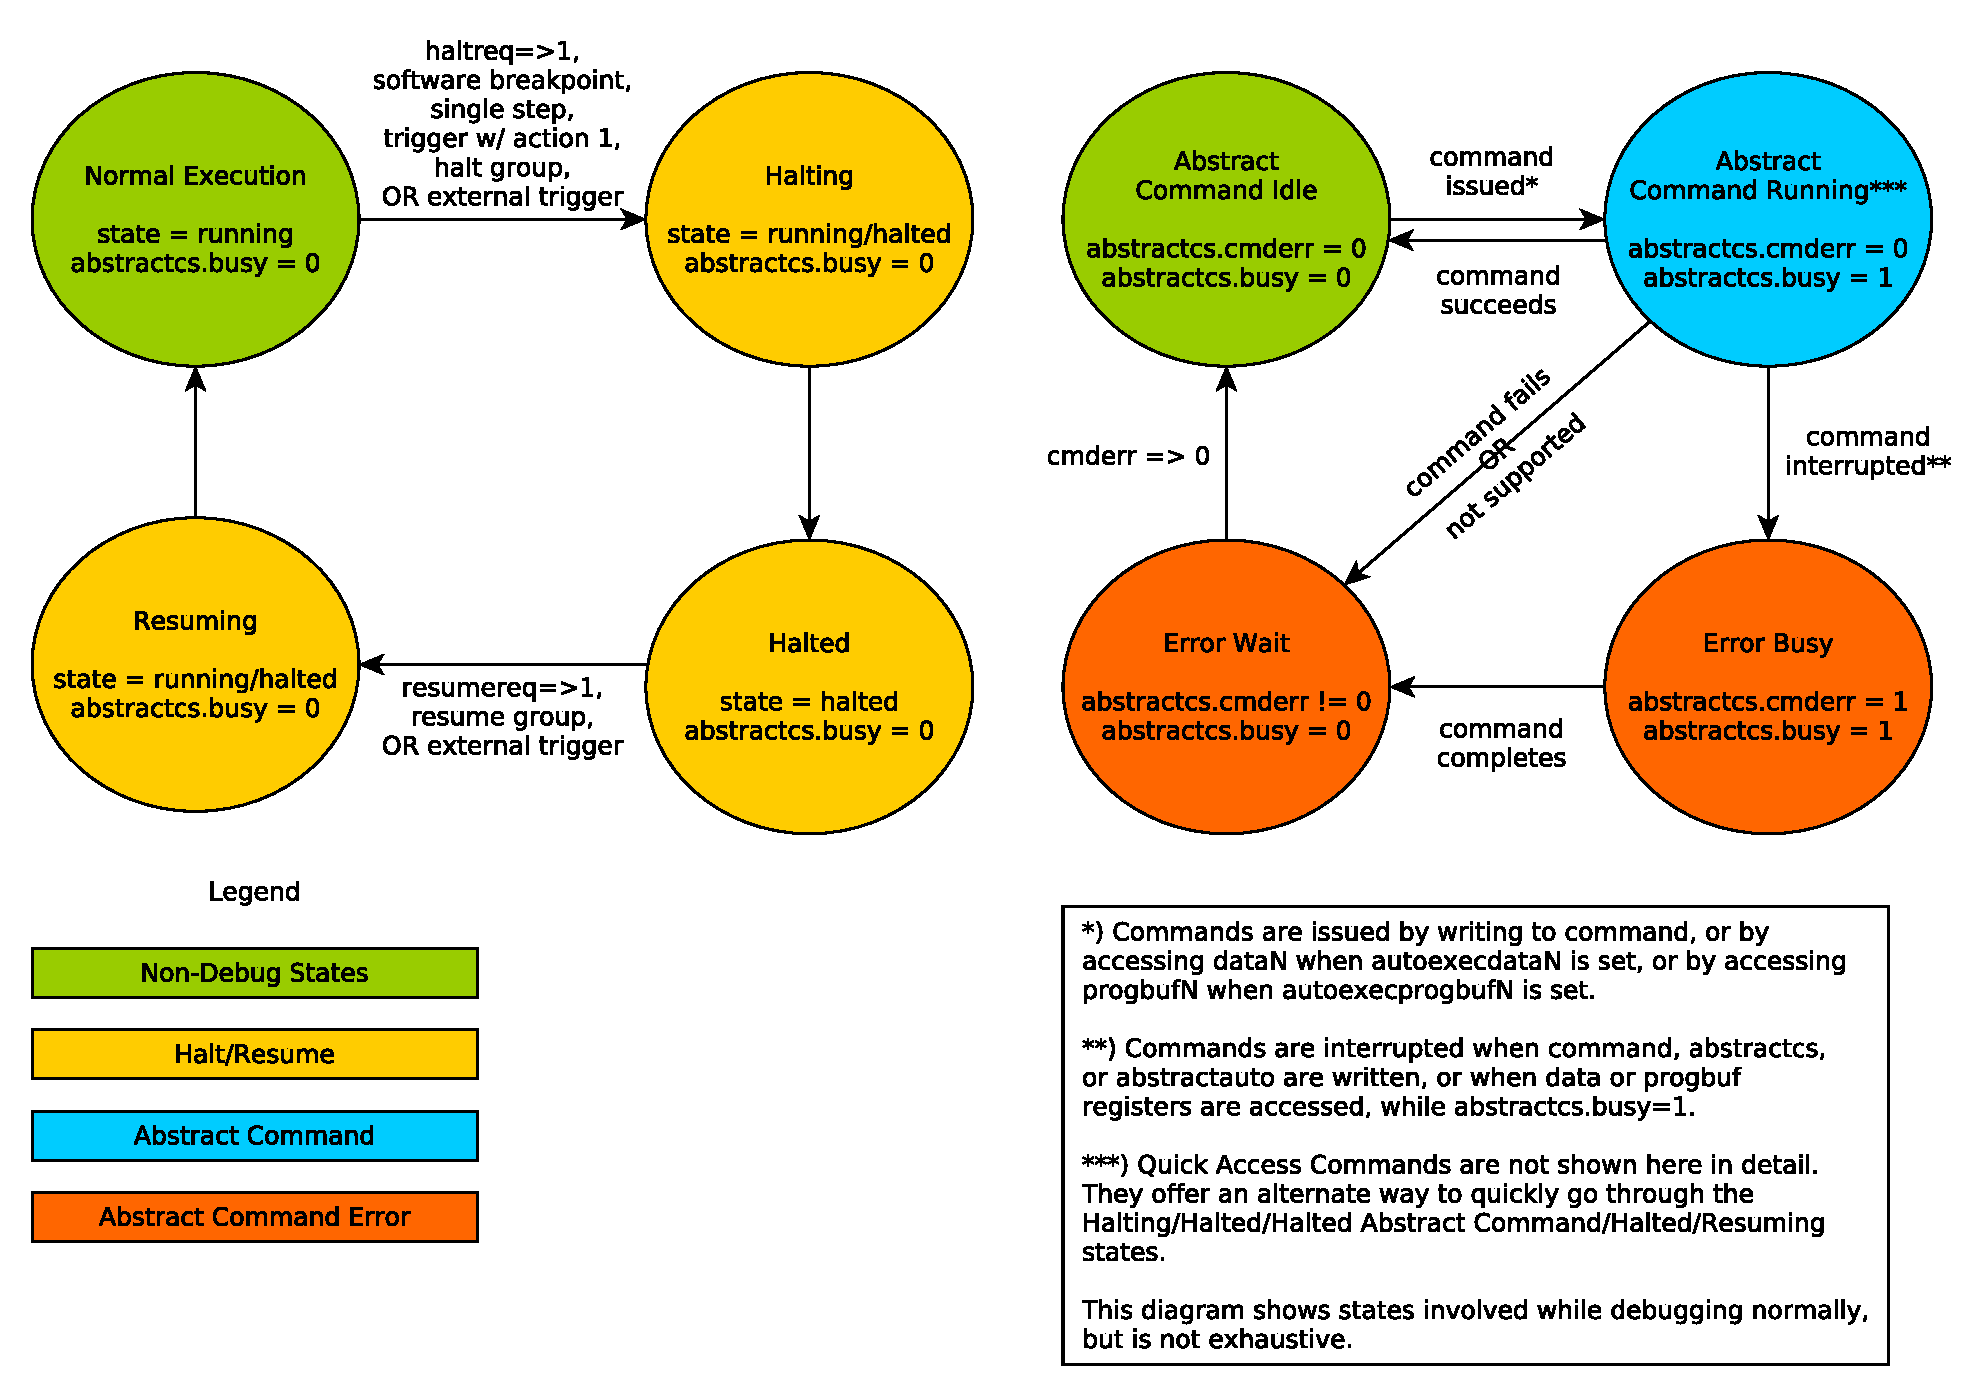
\includegraphics[width=\textwidth]{fig/abstract_commands.pdf}
   \caption[Run/Halt Debug State Machine]{Run/Halt Debug State Machine.
     As only a small amount of state is visibile to the debugger,
     the states and transitions are conceptual.}
   \label{fig:abstract_sm}
\end{figure}

\section{System Bus Access} \label{systembusaccess}

A debugger can access memory from a hart's point of view using a Program Buffer or
the Abstract Access Memory command. (Both these features are optional.)
A Debug Module may also include a System Bus Access block to provide memory
access without
involving a hart, regardless of whether Program Buffer is implemented.
The System Bus Access block uses physical addresses.

The System Bus Access block may support 8-, 16-, 32-, 64-, and 128-bit
accesses. Table~\ref{tab:sbdatabits} shows which bits in {\tt sbdata} are used
for each access size.

\begin{table}[htp]
    \centering
    \caption{System Bus Data Bits}
    \label{tab:sbdatabits}
    \begin{tabulary}{\textwidth}{|r|l|}
        \hline
        Access Size & Data Bits \\
        \hline
        8 & \Rsbdatazero bits 7:0 \\
        \hline
        16 & \Rsbdatazero bits 15:0 \\
        \hline
        32 & \Rsbdatazero \\
        \hline
        64 & \Rsbdataone, \Rsbdatazero \\
        \hline
        128 & \Rsbdatathree, \Rsbdatatwo, \Rsbdataone, \Rsbdatazero \\
        \hline
    \end{tabulary}
\end{table}

Depending on the microarchitecture, data accessed through System Bus Access may
not always be coherent with that observed by each hart. It is up to the
debugger to enforce coherency if the implementation does not. This
specification does not define a standard way to do this, as it is
implementation/platform specific. Possibilities may include
writing to special memory-mapped
locations, or executing special instructions via the Program Buffer.

\begin{commentary}
Implementing a System Bus Access block has several benefits even
when a Debug Module also implements a Program Buffer. 
First, it is possible to
access memory in a running system with minimal impact.  Second, it may improve
performance when accessing memory.
Third, it may provide
access to devices that a hart does not have access to.
\end{commentary}

\section{Quick Access}

Depending on the task it is performing, some harts can only be halted very briefly.
There are several mechanisms that allow accessing resources in such a running system
with a minimal impact on the running hart.

First, an implementation may allow some abstract commands to execute without halting the hart.

Second, the Quick Access abstract command can be used to halt a hart, quickly
execute the contents of the Program Buffer, and let the hart run again.
Combined with instructions that allow Program Buffer code to access the
{\tt data} registers, as described in \ref{hartinfo}, this can be used to quickly
perform a memory or register access. For some systems this will be too
intrusive, but many systems that can't be halted can bear an occasional hiccup
of a hundred or less cycles.

Third, if the System Bus Access block is implemented, it can be used while a
hart is running to access system memory.

\section{Security}

To protect intellectual property it may be desirable to lock access to the
Debug Module.  To allow access during a manufacturing process and not
afterwards, a reasonable solution could be to add a fuse bit to the Debug
Module that can be used to be permanently disable it. Since this is technology
specific, it is not further addressed in this spec.

Another option is to allow the DM to be unlocked only by users who have an
access key. Between \Fauthenticated, \Fauthbusy, and \Rauthdata arbitrarily
complex authentication mechanism can be supported.  When \Fauthenticated is
clear, the DM must not interact with the rest of the platform, nor expose
details about the harts connected to the DM. All DM registers should read 0,
while writes should be ignored, with the following mandatory exceptions:
\begin{steps}{}
    \item \Fauthenticated in \Rdmstatus is readable.
    \item \Fauthbusy in \Rdmstatus is readable.
    \item \Fversion in \Rdmstatus is readable.
    \item \Fdmactive in \Rdmcontrol is readable and writable.
    \item \Rauthdata is readable and writable.
\end{steps}

\section{Debug Module DMI Registers} \label{dmdebbus}

Each DM has a base address (which is 0 for the first DM). The register
addresses described in this section are offsets from this base address.

When read, unimplemented Debug Module DMI Registers return 0. Writing them has
no effect.

For each register it is possible to determine that it is implemented by reading
it and getting a non-zero value (eg. \Rsbcs), or by checking bits in another
register (eg. \Fprogbufsize).

\input{dm_registers.tex}
